\renewcommand\thesection{\arabic{section}}
\renewcommand\thesubsection{\thesection.\arabic{subsection}}
\setcounter{section}{3}
\section{Entrega parcial 4}

\subsection{Se deben incluir al menos 2 funcionalidades propias que sean de utilidad para el negocio (distintas de la inserción, edición, eliminación y reportes)}

Se ha mejorado el menú principal que se encuentra en la clase CLI, dentro del package \textbf{views.cli}, permitiendo funciones específicas de nuestro proyecto como la muestra de información de los alumnos con mejor asistencia, alumnos entre cierto porcentaje de asistencia o retiro.

\Shell{Menú asistencia}{contents/code/salida11.txt}

\subsubsection{Seleccionar un objeto por criterio, considera la selección de un objeto basado en un criterio específico, involucrando dos o más colecciones anidadas. Por ejemplo, selección del alumno con la nota final más baja de todos los cursos, o seleccionar el pasajero más joven de todos los buses de una compañía}

El sistema permite obtener los datos del alumno que registra más retiros durante un año escolar, mediante el menú asistencia, opción 4.

\subsubsection{Subconjunto filtrado por criterio: considera la selección de un subconjunto de objetos basado en un criterio específico, involucrando dos o más colecciones anidadas. Por ejemplo, selección de los alumnos con nota final entre 4,0 y 7,0 de entre todos los cursos; o seleccionar a todos los pasajeros que tengan asiento impar de entre todos los buses de la compañía}

El sistema permite obtener los datos de aquellos alumnos que estén entre un rango (porcentaje) de asistencia o retiros definido por el usuario, mediante el menú asistencia, opciones 3 y 5.

\subsection{Diseño y codificación de 2 (dos) clases que utilicen sobreescritura de métodos}

Las clases que hemos diseñado y codificado con métodos de sobre escritura son aquellas que poseen colección en el package \textbf{database} y \textbf{datafile}.

\begin{figure}[h]
    \centering
    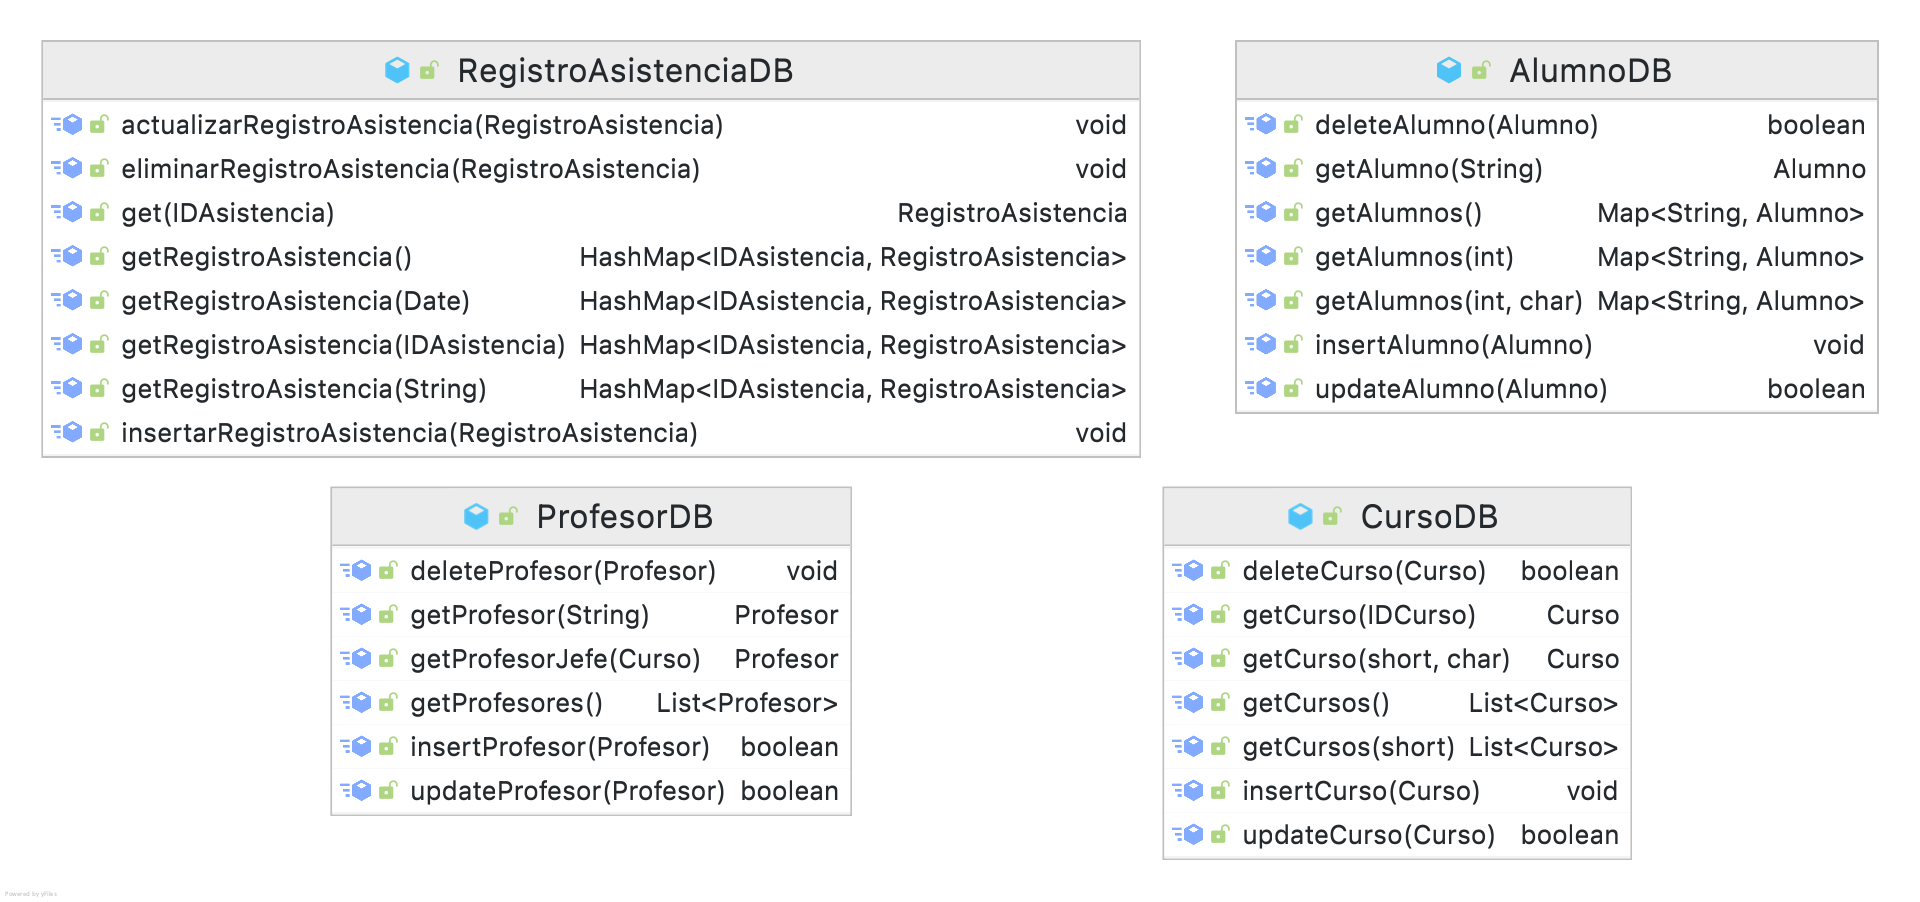
\includegraphics[width=0.6\textwidth]{contents/img/img8}
    \caption{Métodos paquete Database}
    \label{fig:img8}
\end{figure}

\clearpage

\begin{figure}[h]
    \centering
    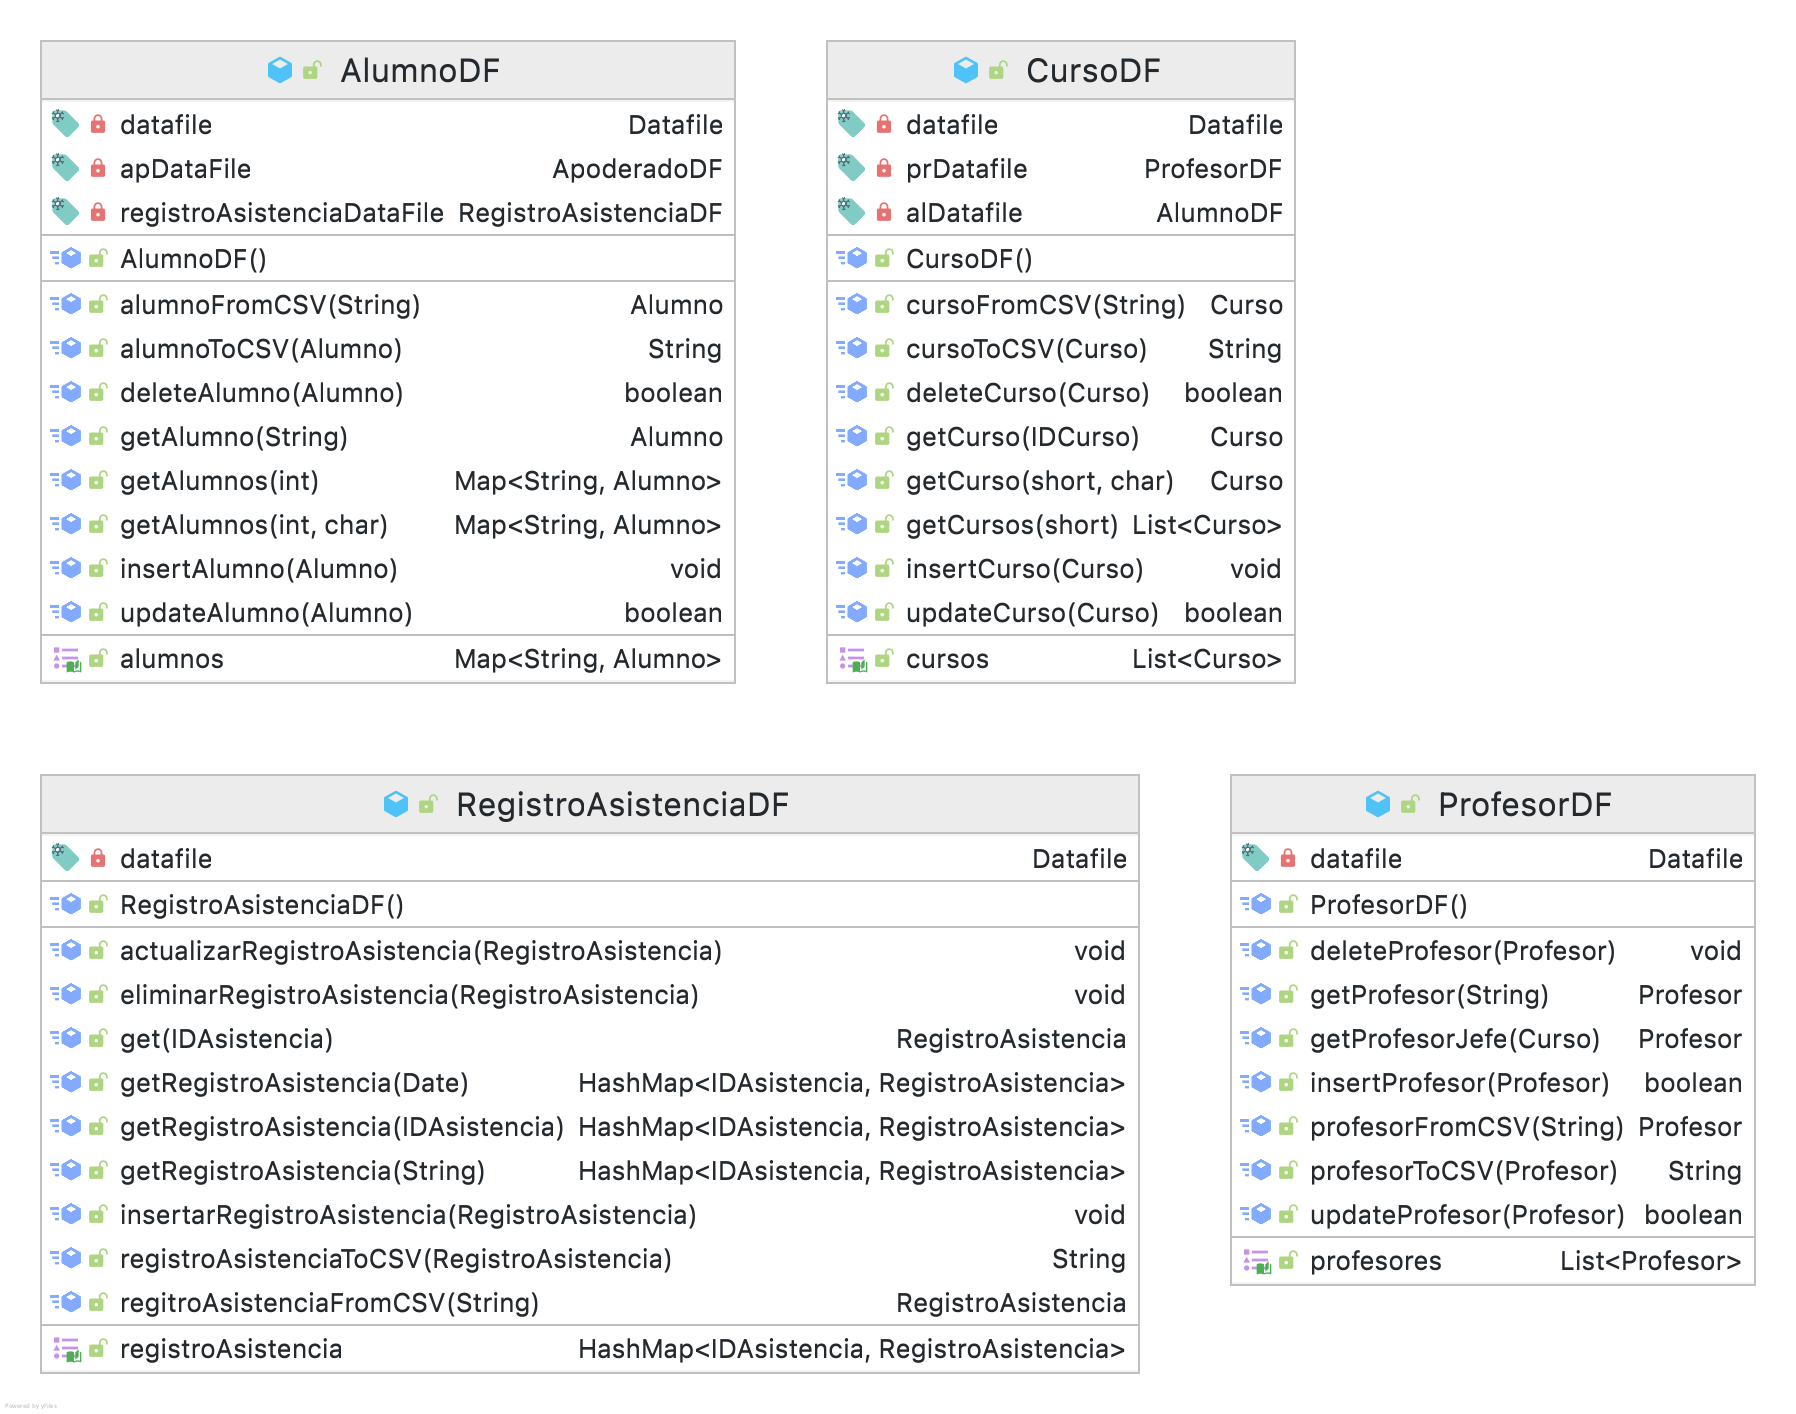
\includegraphics[width=0.75\textwidth]{contents/img/img9}
    \caption{Métodos paquete Datafile}
    \label{fig:img9}
\end{figure}

\subsection{Diseño y codificación de 1 (una) clase abstracta que sea padre de al menos 2 (dos) clases. La clase abstracta debe ser utilizada por alguna otra clase (contexto)}

La clase abstracta codificada es la \textbf{Persona} que posee las características: rut, nombres, apellido paterno y apellido materno, las cuales son pasadas a sus hijos.

\begin{figure}[h]
    \centering
    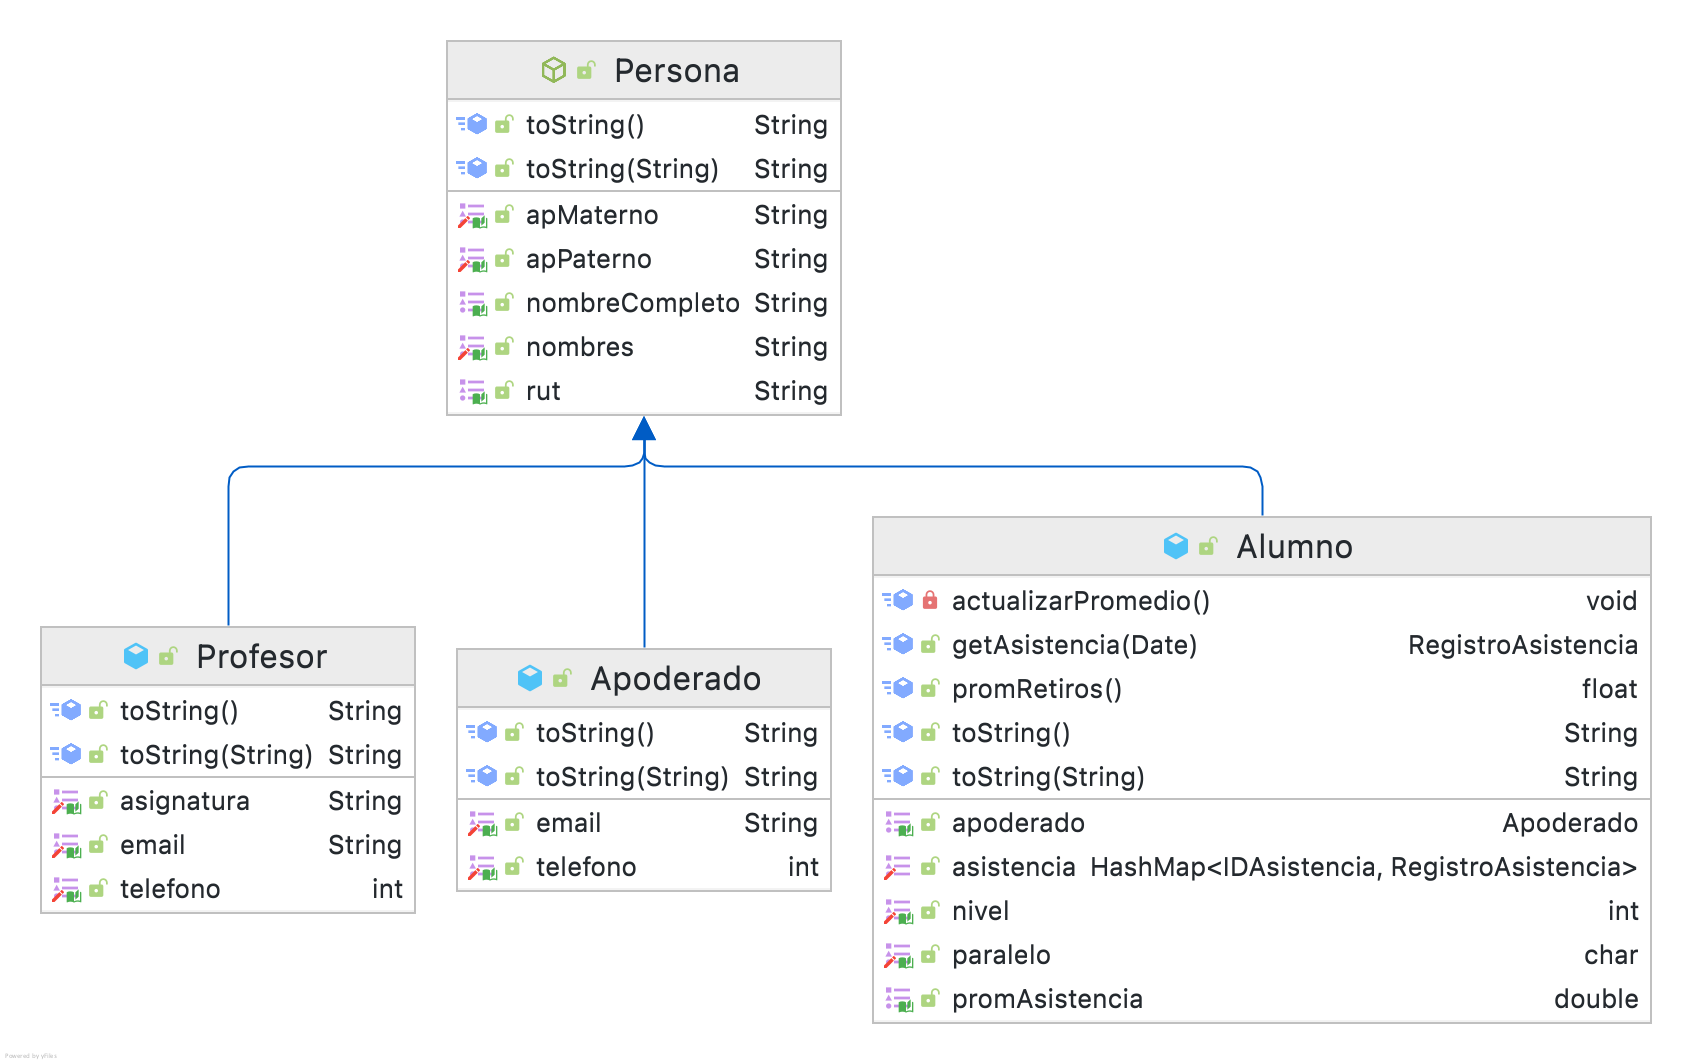
\includegraphics[width=0.5\textwidth]{contents/img/img10}
    \caption{Clase abstracta Persona y sus clases hijas}
    \label{fig:img10}
\end{figure}

\clearpage

\subsection{Diseño y codificación de 1 (una) interfaz que sea implementada por al menos 2 (dos) clases. La interfaz debe ser utilizada por alguna otra clase (contexto)}

Las interfaz diseñadas son al igual que en el punto 2 aquellas que poseen colección el package \textbf{database} y \textbf{datafile}. El diseño de la interfaz, en conjunto con el patrón de diseño \textit{Strategy}, permite la independencia del sistema al origen de datos, pudiendo cambiar este último sin inconvenientes, mientras implemente los métodos descritos en las interfaces presentes en el package \textbf{Data}.

\begin{figure}[h]
    \centering
    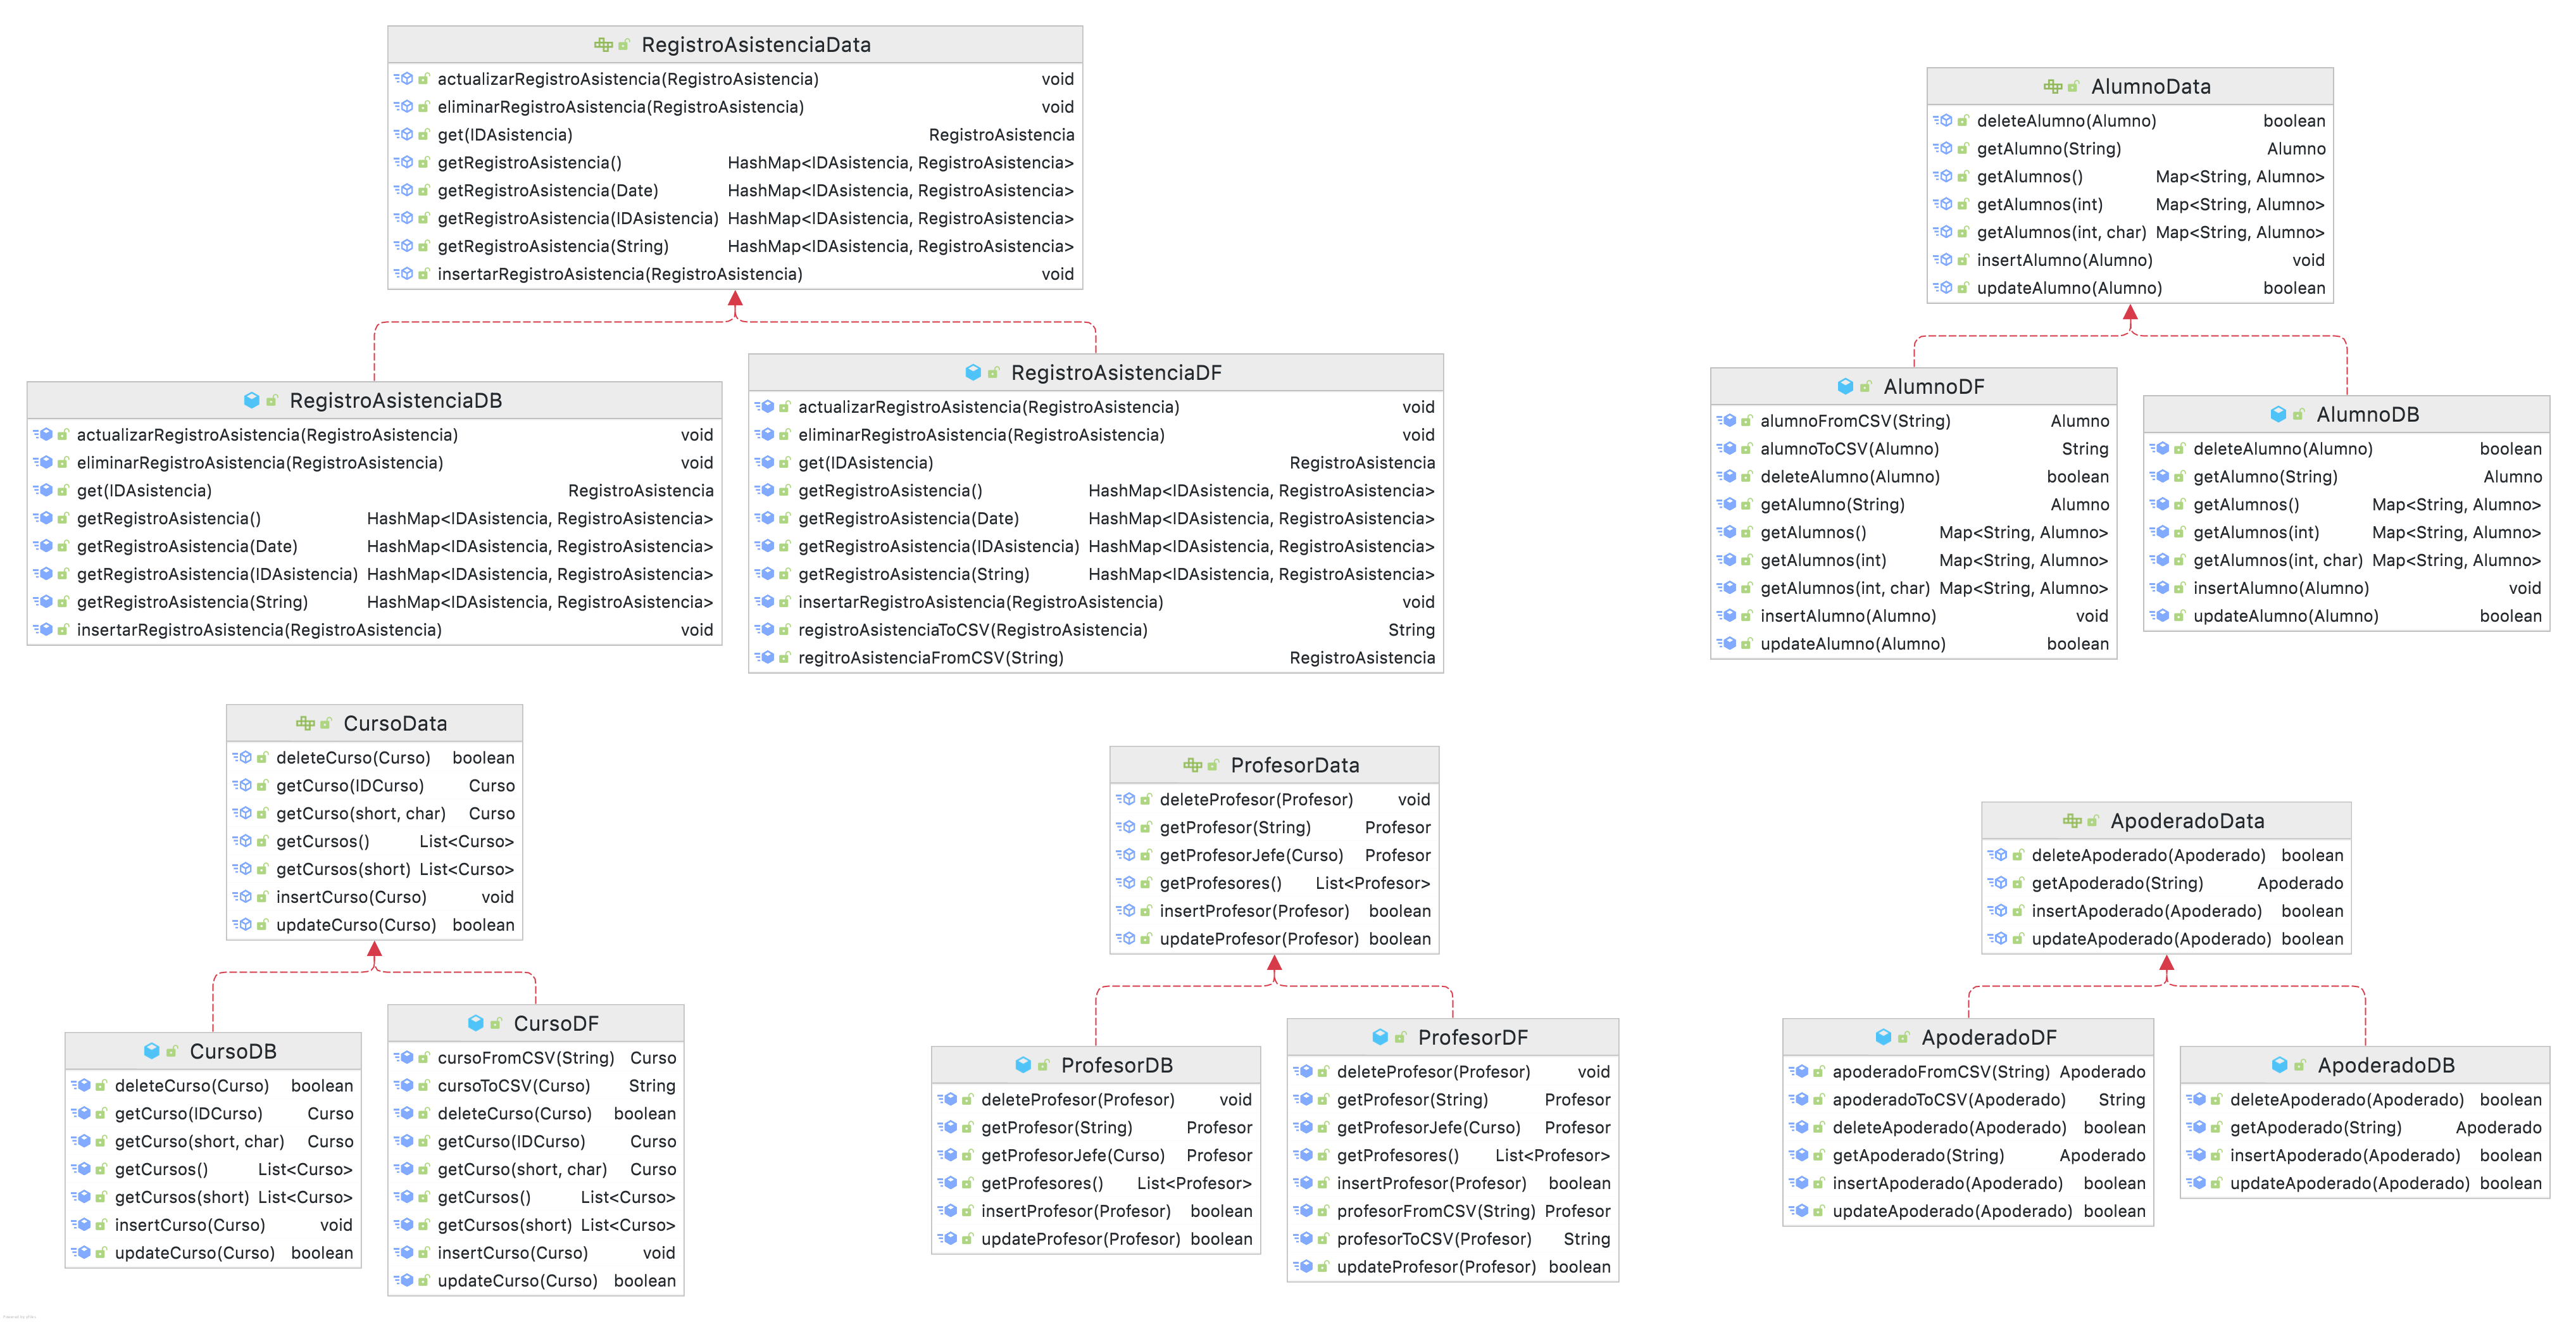
\includegraphics[width=0.85\textwidth]{contents/img/img11}
    \caption{Interfaces Data y sus implementaciones}
    \label{fig:img11}
\end{figure}

\subsubsection*{Opcional: Generar documentación con Javadoc.}
\addcontentsline{toc}{subsubsection}{Opcional: Generar documentación con Javadoc.}

Lorem ipsum dolor sit amet, consectetur adipiscing elit. Donec et sem luctus, finibus mauris eget, euismod arcu. Morbi at mollis risus. Praesent consequat justo tellus, ac pretium urna lacinia quis. Ut sagittis cursus finibus. Morbi pellentesque vulputate tincidunt. Aliquam at pretium tellus, et vehicula velit. Nunc turpis metus, porttitor sit amet aliquam ut, venenatis quis elit. Nam tincidunt venenatis tortor, ac sodales libero varius nec. Donec vestibulum leo a metus rutrum, vitae elementum diam suscipit. Quisque non mauris rutrum, lacinia lectus id, viverra dui. In leo quam, ultrices vitae suscipit quis, porttitor quis turpis. Vestibulum semper ligula sit amet diam scelerisque gravida.

